\documentclass[12pt]{article}
\usepackage[spanish,mexico]{babel}
	\selectlanguage{spanish}
\usepackage{graphicx}
\usepackage{amsmath}
\usepackage{wrapfig}
\usepackage{float}
\usepackage[utf8]{inputenc}
\usepackage{hyperref}
\usepackage{graphicx}
\graphicspath{{images/}}

\usepackage{vmargin}
\setmarginsrb{3 cm}{0.25 cm}{3 cm}{0.25 cm}{1 cm}{1.5 cm}{1 cm}{1.5 cm}
\usepackage{listings}
\usepackage[usenames,dvipsnames]{color}
	\definecolor{ocre}{RGB}{42,105,21}
	\definecolor{ocre2}{RGB}{47,109,130}
	\definecolor{gray2}{gray}{0.95}
	\lstset{
		language=Python,
		backgroundcolor=\color{gray2},
		basicstyle=\color{black}\small\ttfamily, 
		breakatwhitespace=false,         
		breaklines=true,                 
		captionpos=b,                    
		columns=flexible,
		commentstyle=\color{ocre2}\ttfamily, 
		deletekeywords={...},            
		escapeinside={\%*}{*)},          
		extendedchars=true,             
		frame=single,	                 
		keepspaces=true,                 
		keywordstyle=\color{blue}\bfseries,       
		otherkeywords={*,...},          
		numbers=left,                    
		numbersep=5pt,                   
		numberstyle=\tiny, 
		rulecolor=\color{black},         
		showspaces=false,                
		showstringspaces=false,          
		showtabs=false,                  
		stepnumber=1,                    
		stringstyle=\normalfont\color{ocre},     
		tabsize=2,	                     
		title=\lstname                  
		}

\title{Actividad 10: Animaciones con Matplotlib}
\author{Martin Alejandro Paredes Sosa}
\date{Marzo, 2016}

\begin{document}
\maketitle

\section{Introducción}
\noindent
Un zombie\cite{Wiki} es un termino asociado a una persona infectada por un virus que básicamente se aloja en el cerebro y apaga los sistemas internos de la victima, transformándolos en muertos vivientes. Por otra parte, un zombie es un cuerpo reanimado que se alimenta de carne humana. Las historias sobre zombies, son tan antiguas como la raza humana. 

\begin{figure}[H]
\centering

\includegraphics[scale=0.25]{zom.jpg}
%\caption{Ejemplo Zombie}
\end{figure}

Para esta actividad, se nos pidió recrear la gráficas de un modelo de apocalipsis zombie basándonos del articulo de Philip Munz\cite{Manual} sobre un modelo matemático sobre un brote de infección zombie. Este articulo explica los conceptos básicos que se deben tomar en cuenta para modelar un apocalipsis zombie.

\pagebreak
%===============================================================================
%===============================================================================
\section{Modelo Zombie}
Para entender los modelos, explicaremos la bases de estos basándonos en el articulo del modelo zombie \cite{Manual}:
\subparagraph{Clases:}
\begin{itemize}
	\item \textbf{S:} Población susceptible a infectarse o morir, es decir, los vivos.
	\item \textbf{Z:} Población Zombie
	\item \textbf{R:} Población de individuos removidos o eliminados.
	\item \textbf{I:} Población de infectados pero no zombies.
	\item \textbf{Q:} Población en cuarentena.
\end{itemize}
La dinámica en general es la siguiente:
\begin{itemize}
	\item \textbf{S} puede aumentar si consideramos natalidad y disminuye por infectados o muerte por causa natural.
	\item \textbf{Z} aumenta por la cantidad de infectados y muertes y disminuye si la población es curada o se encuentra en cuarentena.
	\item \textbf{R} aumenta por la muertes en enfrentamientos zombies y humanos, muerte natural o por la cuarentena. Disminuye si resucitan como zombies.
	\item \textbf{I} aumentan con el tiempo y disminuyen si se transforman, mueren, los curan o son enviados a cuarentena.
	\item \textbf{Q} aumenta con los infectados y zombies que son enviados a cuarentena y disminuye si mueren.
\end{itemize}

Existen muchos parámetros que pueden influir en la dinámica de la población los definimos de la siguiente manera:

\begin{itemize}
	\item $\prod$: Tasa de natalidad.
	\item $\delta$: Tasa de muertes naturales.
	\item $\beta$: Tasa de transmisión.
	\item $\zeta$: Tasa de resucitación.
	\item $\alpha$: Tasa de destrucción \textbf{Z}.
	\item $\rho$: Tasa de conversión de \textbf{I} a \textbf{Z}.
	\item $\kappa$: Tasa de ingreso de \textbf{I} a \textbf{Q}.
	\item $\sigma$: Tasa de ingreso de \textbf{Z} a \textbf{Q}.
	\item $\gamma$: Tasa de muertes en \textbf{Q}.
	\item $c$: Tasa de cura.
\end{itemize}
Una vez establecido las clases, sus dinámicas y los parametros que los afectan, se puede empezar a analizar los diversos modelos del articulo.

%===============================================================================
\subsection{Modelo Básico (SZR)}
En este modelo se consideran solamente a las clases \textbf{S}, \textbf{Z} y \textbf{R}. Donde los sanos se pueden convertir en zombies perdiendo en un encuentro con un zombie. Se puede evitar la transformación eliminando zombies. Los removidos consiste de individuos muertos, los cuales pueden resurgir como zombies.

\textbf{Ecuaciones del Modelo Básico}
\begin{figure}[H]
\centering
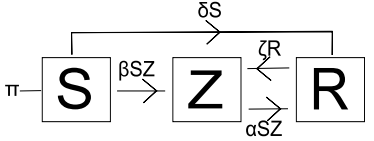
\includegraphics[scale=0.5]{ModeloG.png}
\hspace{0.5cm}
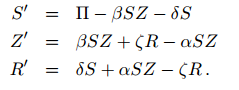
\includegraphics[scale=0.65]{Modelo.png}
\end{figure}

Las siguientes gráficas son los resultados de esto modelo:
\begin{figure}[H]
\centering
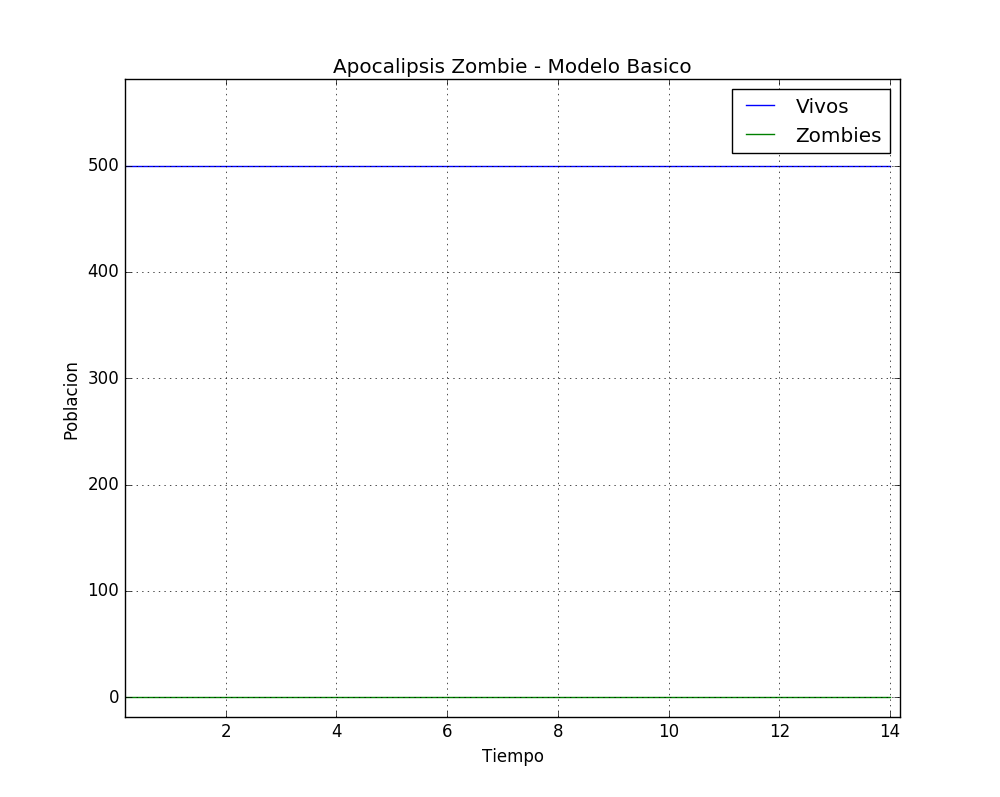
\includegraphics[height=7.5cm]{BasicoE.png}
\caption{Caso sin zombies SZR}
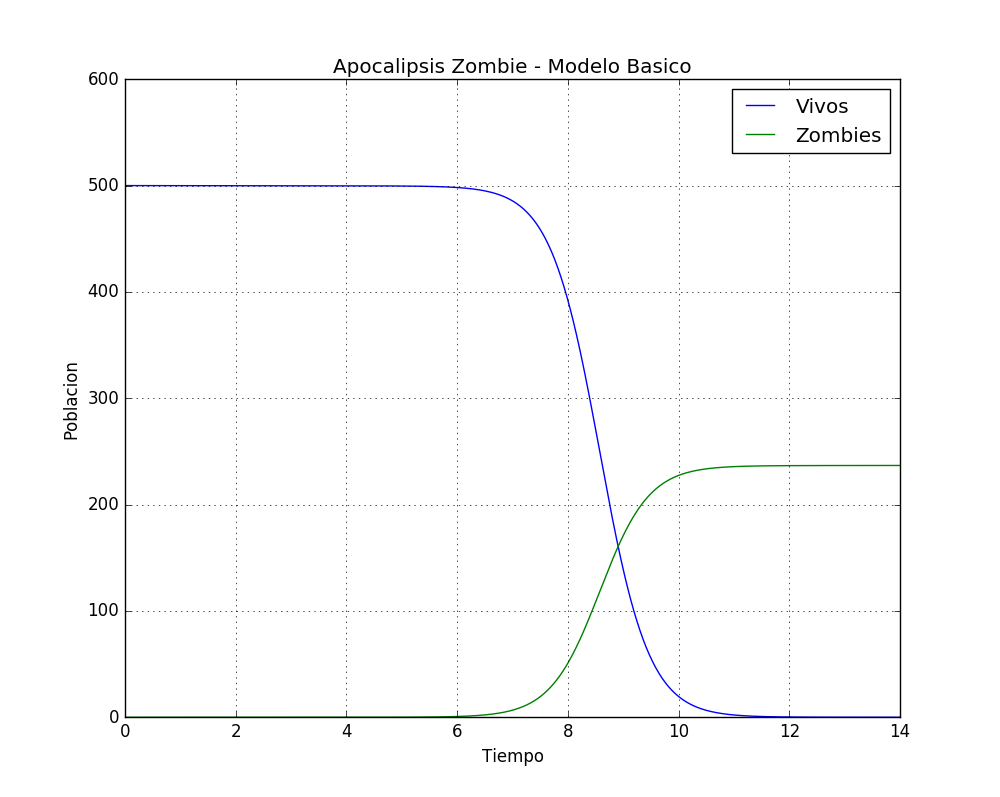
\includegraphics[height=7.5cm]{BasicoR.png}
\caption{Modelo Básico SZR}
\end{figure} 

%===============================================================================
\subsection{Modelo con Infección Latente (SIZR)}
Ahora tenemos un modelo que incluye el efecto de una clase de infectados. Si consideramos un tiempo de incubación y el efecto del virus en alguien infectado, se puede pensar en una tasa de conversión. Esta nueva clase modifica a la población \textbf{Z} de manera directa, lo cual retarda el tiempo en el que \textbf{S} se transforma a la clase \textbf{Z}.

\textbf{Ecuaciones del Modelo con Infección Latente}
\begin{figure}[H]
\centering
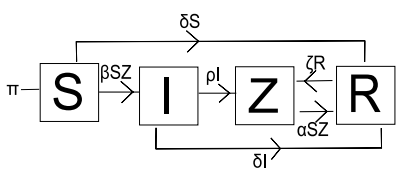
\includegraphics[scale=0.5]{LModeloG.png}
\hspace{0.5cm}
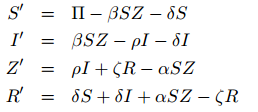
\includegraphics[scale=0.65]{LModelo.png}
\end{figure}

Las siguientes gráficas son los resultados de esto modelo:
\begin{figure}[H]
\centering
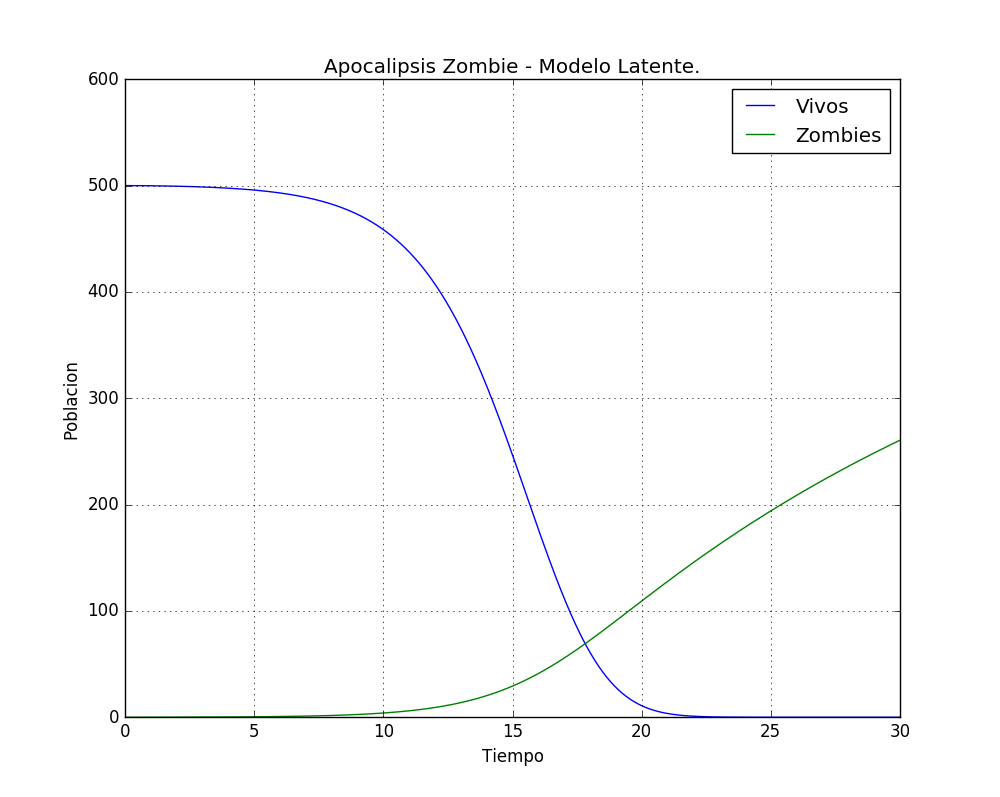
\includegraphics[height=7.5cm]{Latente.png}
\caption{Modelo Básico SIZR}
\end{figure} 
\pagebreak

%===============================================================================
\subsection{Modelo con Cuarentena (SIZRQ)}
Para contener el brote, la población separa a los infectados y los pone en cuarentena, así como a una cierta de la población zombie. Pero, los individuos en cuarentena internan escapar y son eliminados antes de lograrlo, o bien mueren en cuarentena.

\textbf{Ecuaciones del Modelo con Cuarentena}
\begin{figure}[H]
\centering
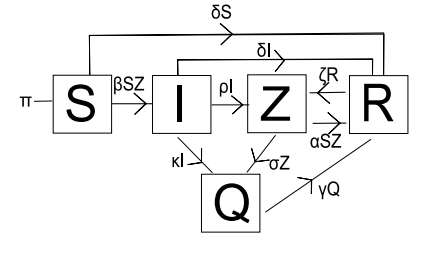
\includegraphics[scale=0.45]{QModeloG.png}
\hspace{0.5cm}
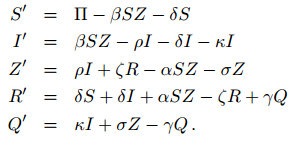
\includegraphics[scale=0.65]{QModelo.png}
\end{figure}

Las siguientes gráficas son los resultados de esto modelo:
\begin{figure}[H]
\centering
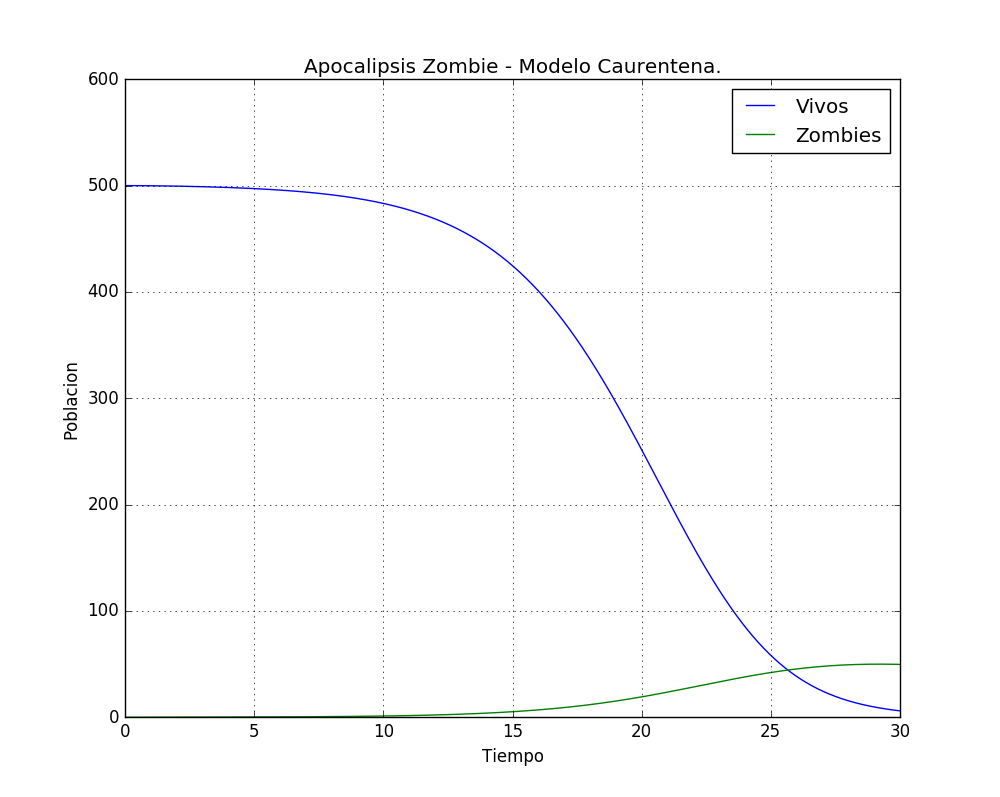
\includegraphics[height=7.5cm]{Cuarentena.png}
\caption{Modelo Básico SIZRQ}
\end{figure} 
\pagebreak

%===============================================================================
\subsection{Modelo con Cura}
Supongamos que podamos producir rápidamente una cura. Este tratamiento permitiría transformar a los zombies en humanos. Pero la cura no los vuelve inmunes. Con la cura ya no se tiene la necesidad de tener la cuarentena para los infectados.

\textbf{Ecuaciones del Modelo con Cura}
\begin{figure}[H]
\centering
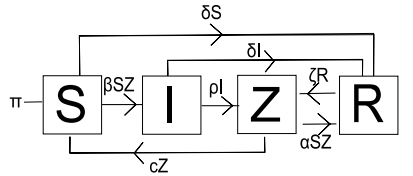
\includegraphics[scale=0.5]{CModeloG.png}
\hspace{0.5cm}
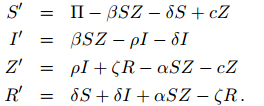
\includegraphics[scale=0.65]{CModelo.png}
\end{figure}

Las siguientes gráficas son los resultados de esto modelo:
\begin{figure}[H]
\centering
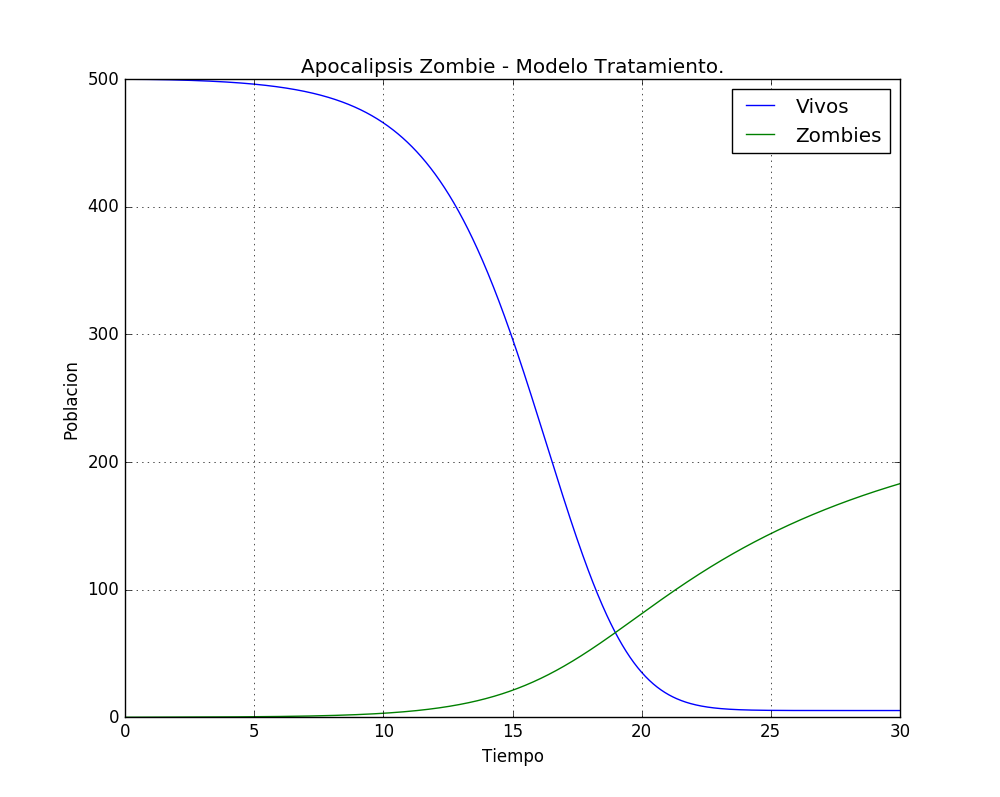
\includegraphics[height=7.5cm]{Tratamiento.png}
\caption{Modelo Básico SIZR con cura}
\end{figure} 
\pagebreak

%===============================================================================%===============================================================================
\section{Códigos}
A continuación se mostraran los códigos que se utilizaron.
\subsection{Modelo Básico}
\lstinputlisting[caption={Código Modelo\_Basico.py}]{Modelo_Basico.py}

\subsection{Modelo con Infección Latente}
\lstinputlisting[caption={Código Latente.py}]{Latente.py}

\subsection{Modelo con Cuarentena}
\lstinputlisting[caption={Código Cuarentena.py}]{Cuarentena.py}

\subsection{Modelo con Cura}
\lstinputlisting[caption={Código Tratamiento.py}]{Tratamiento.py}
%===============================================================================%===============================================================================



%\lstinputlisting[caption={Código Animacion\_Pendulo.py}]{Cuarentena.py}
\pagebreak
\begin{thebibliography}{6}
\bibitem{Wiki}
	Zombiepedia,(2016)
	\emph{Zombies}. Recuperado de: \url{http://zombie.wikia.com/wiki/Special:WikiActivity}

\bibitem{Manual}
	Munz, P., Hudea, I., Imad, J., et al(2009)
	\emph{When zombies attack!: Mathematical modelinng of an outbreak of zombie infection} Recuperado de: \url{http://mysite.science.uottawa.ca/rsmith43/Zombies.pdf}

\bibitem{Codigo}
	Scipy Cookbook.(2015)
	\emph{Modeling a Zombie Apocalypse} Recuperado de: \url{http://scipy-cookbook.readthedocs.io/items/Zombie\_Apocalypse\_ODEINT.html}


\bibitem{Actividad}
	Lizárraga, C. (2016)
	\emph{Actividad 11 (2016-1)}. Recuperado de \url{http://computacional1.pbworks.com/w/page/107502219/Actividad\%2011\%20\%282016-1\%29}
\end{thebibliography}

\end{document}